\documentclass[twocolumn,9pt,a4paper]{jsarticle}
%
\usepackage{amsmath,amssymb}
\usepackage{bm}
\usepackage{epsbox}
\usepackage[dvipdfmx]{graphicx}
\usepackage{verbatim}
\usepackage{wrapfig}
\usepackage{ascmac}
\usepackage{makeidx}
\usepackage[dvipdfmx]{graphicx}

\usepackage{listings, jlisting}
\usepackage{color}
 
\lstset{
    language=Python,%プログラミング言語によって変える。
    numbers = left,
    numberstyle = {\tiny \emph},
    numbersep = 10pt,
    breaklines = true,
    breakindent = 40pt,
    frame = tlRB,
    frameround = ffft,
    framesep = 3pt,
    rulesep = 1pt,
    rulecolor = {\color{black}},
    rulesepcolor = {\color{black}},
    flexiblecolumns = true,
    keepspaces = false,
    basicstyle = \scriptsize,
    identifierstyle = \itshape\scriptsize,
    commentstyle = \fontfamily{ptm}\selectfont\scriptsize,
    stringstyle = \scshape\scriptsize,
    tabsize = 4, 
 }

%
\setlength{\textwidth}{\fullwidth}
%\setlength{\textheight}{40\baselineskip}
\addtolength{\textheight}{\topskip}
\setlength{\voffset}{-0.2in}
\setlength{\topmargin}{0pt}
%\setlength{\headheight}{0pt}
%\setlength{\headsep}{0pt}
%
\newcommand{\divergence}{\mathrm{div}\,}  %ダイバージェンス
\newcommand{\grad}{\mathrm{grad}\,}  %グラディエント
\newcommand{\rot}{\mathrm{rot}\,}  %ローテーション
%
\title{Scratchプログラムの可視化による類似度推定}
\author{G13924 森下汐美 G13908 岩科智彩}
\date{平成29年1月31日}
\begin{document}
\maketitle
%
%
\section{はじめに}
近年プログラミング教育が推進され、日本でも小学校での導入が検討されている。子供のプログラミング教育の方法として近年よく利用されているのが米国マサチューセッツ工科大学のメディアラボが開発したScratchである。ScratchとはGUI環境を提供し、ブロックを組み合わせることでプログラムを作る。初心者にとっては使いやすい設計となっているため米国では利用者が増えている。また利用者同士ではプログラムを公開し共有するためのサイトも提供している。そこで実際にサイトで公表されているScratchプログラムを利用して、教育を支援するツールを目指すことにした。Scratchではあるプログラムが引用された場合、その関係をリミックスツリーという図で表している。これでは引用関係は分かるが実際に引用されたもの同士の類似度は表されていないため、一箇所の変更を加えたもの、多数の変更を加えたものはリミックスツリー上では引用元のプロジェクトから同距離で表されている。本研究ではリミックスツリー上では表されていない類似性の数値化を行い、より分かりやすく表示させることを目指した。
\section{Scratchの現状}
Scratchプロジェクトではあるプログラムが引用された場合、その関係をリミックスツリーという図で表している。これでは引用関係は分かるが実際に引用されたもの同士の類似度は表されていないため、一箇所の変更を加えたもの、多数の変更を加えたものはリミックスツリー上では引用元のプロジェクトから同距離で表されている。この距離が数値化され、分かりやすく表されれば、例えば生徒の課題が提出された際にサンプルプログラムとの類似性で評価が分かりやすくできるのではないかと考える。
\section{提案する手法}
本研究では2つのプログラムと1つの辞書データを使用する。Python環境ではjsonモジュールをインポートすることでJSON形式ファイルを読み込み辞書型に変換されるためPythonで計算プログラムを作成し、JSON形式でインポートしたScratchプログラムを解析する。
類似度尺度はcos類似度を用いる。cos類似度とはベクトル空間モデルにおいて、文書同士を比較する際に用いられる類似度計算方法である。
\\【数式】
\begin{equation}
\cos(A,B) = \frac{\vec{A} \ast\vec{B}} {|\vec{A}||\vec{B}|}  = \frac{\vec{A}}{|\vec{B}|}\ast\frac{\vec{A}}{|\vec{B}|} = \frac{\sqrt {\sum_{i=1}^{|V|}}}{\sqrt{\sum_{i=1}^{|V|}A_i^2\ast\sum_{i=1}^{|V|}B_i^2}}
\end{equation}
Scratchでは数多くのブロックが用意されており、どのブロックを使用するかによって、まったく異なるプログラムを作成することができるため本研究ではブロックの種類ごとの個数を集計をした後、ソートしたものをベクターに直し計算式に適用する。
\\ブロック数とスプライト数はJSON形式データの操作をPythonで行うプログラムを用意し、計算する。
\section{実験方法}
本研究では2万弱の引用がされている"Pong Starter"のプロジェクトのリミックスツリーを利用し、各プロジェクトの元のプロジェクトと比較をしていき、 使われたブロックの数、スプライト(オブジェクト)の数、類似度を表すcos類似度の数値化、グラフ化をする。まず元のプログラムから引用されたものを1段目とする。以後1段目のプロジェクトから引用されたもの を2段目、2段目から引用されたものを3段目とし、各段ごとにグラフを作成する。
\section{実験結果}
出力されたデータを用いて散布図に表した。縦軸にcos類似度の値、横軸に出力されたブロック数(スプライト数)を元のプログラム("Pong Starter")の数値で割った値の対数値でとる。数値では(1,1)が最も類似しているプロジェクトであるため似ているものから青、赤、緑、紫、水色で色を区別してプロットをする。カラーマップでは各要素の個数を集計し、頻度の高いものから色別でプロットした。
\\
\subsection{ブロック数とcos類似度の散布図}
\begin{figure}[h]
 \begin{tabular}{cc}
 	\begin{minipage}[t]{0.45\hsize}
	 \centering
	 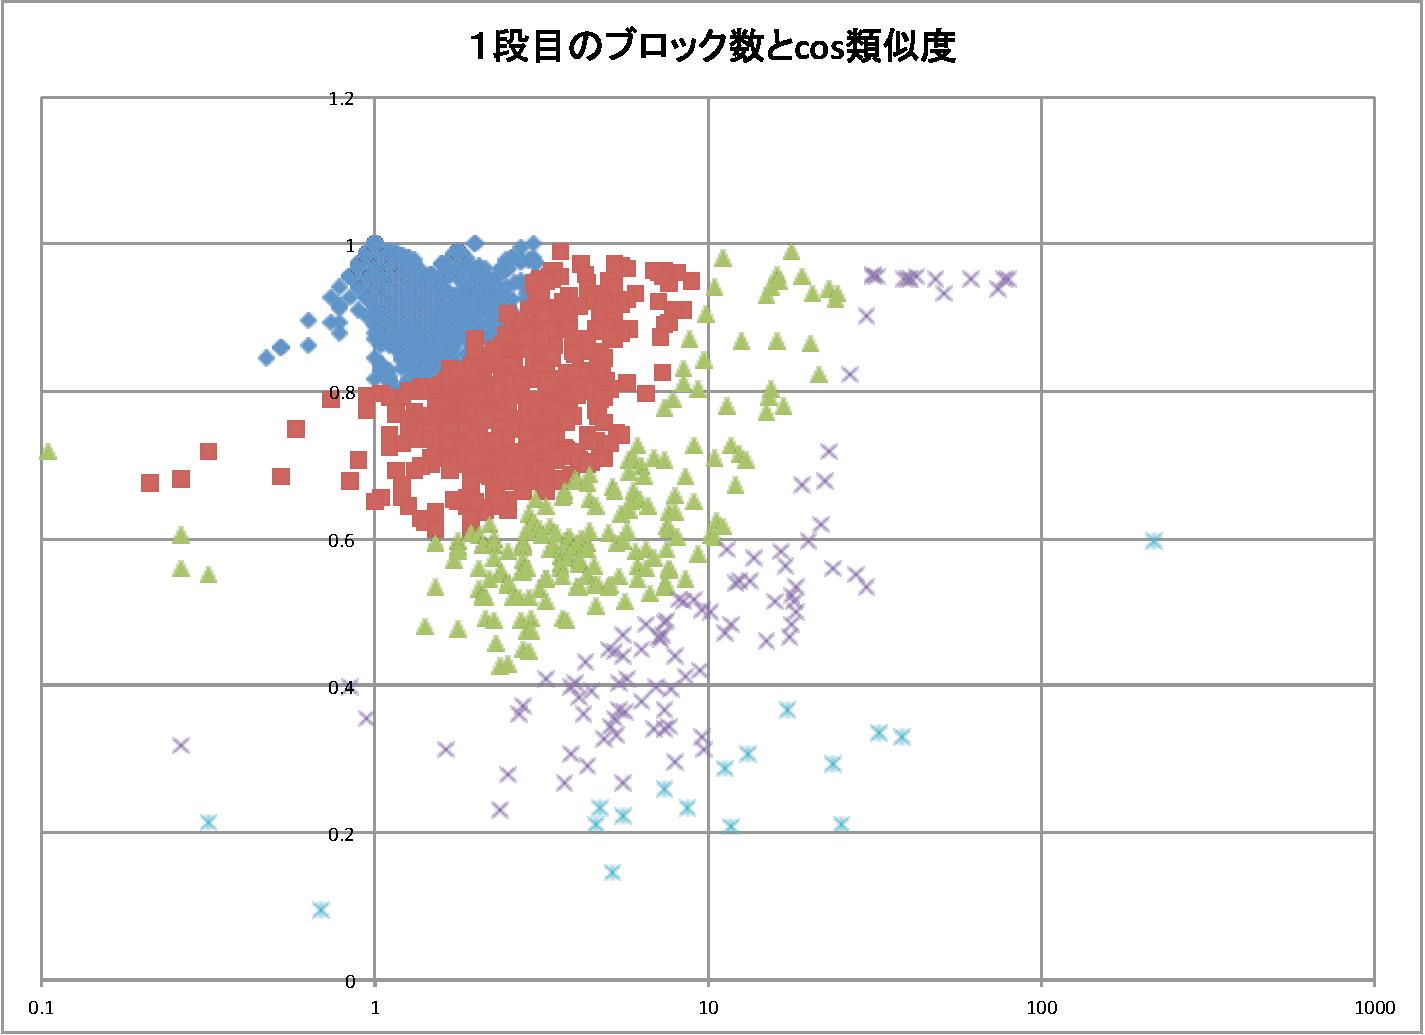
\includegraphics[keepaspectratio, scale = 0.15]{graph_1_block.pdf}
	 \caption{1段目のグラフ}
	 \label{first_block}
	\end{minipage}
        \begin{minipage}[t]{0.45\hsize}
	 \centering
	 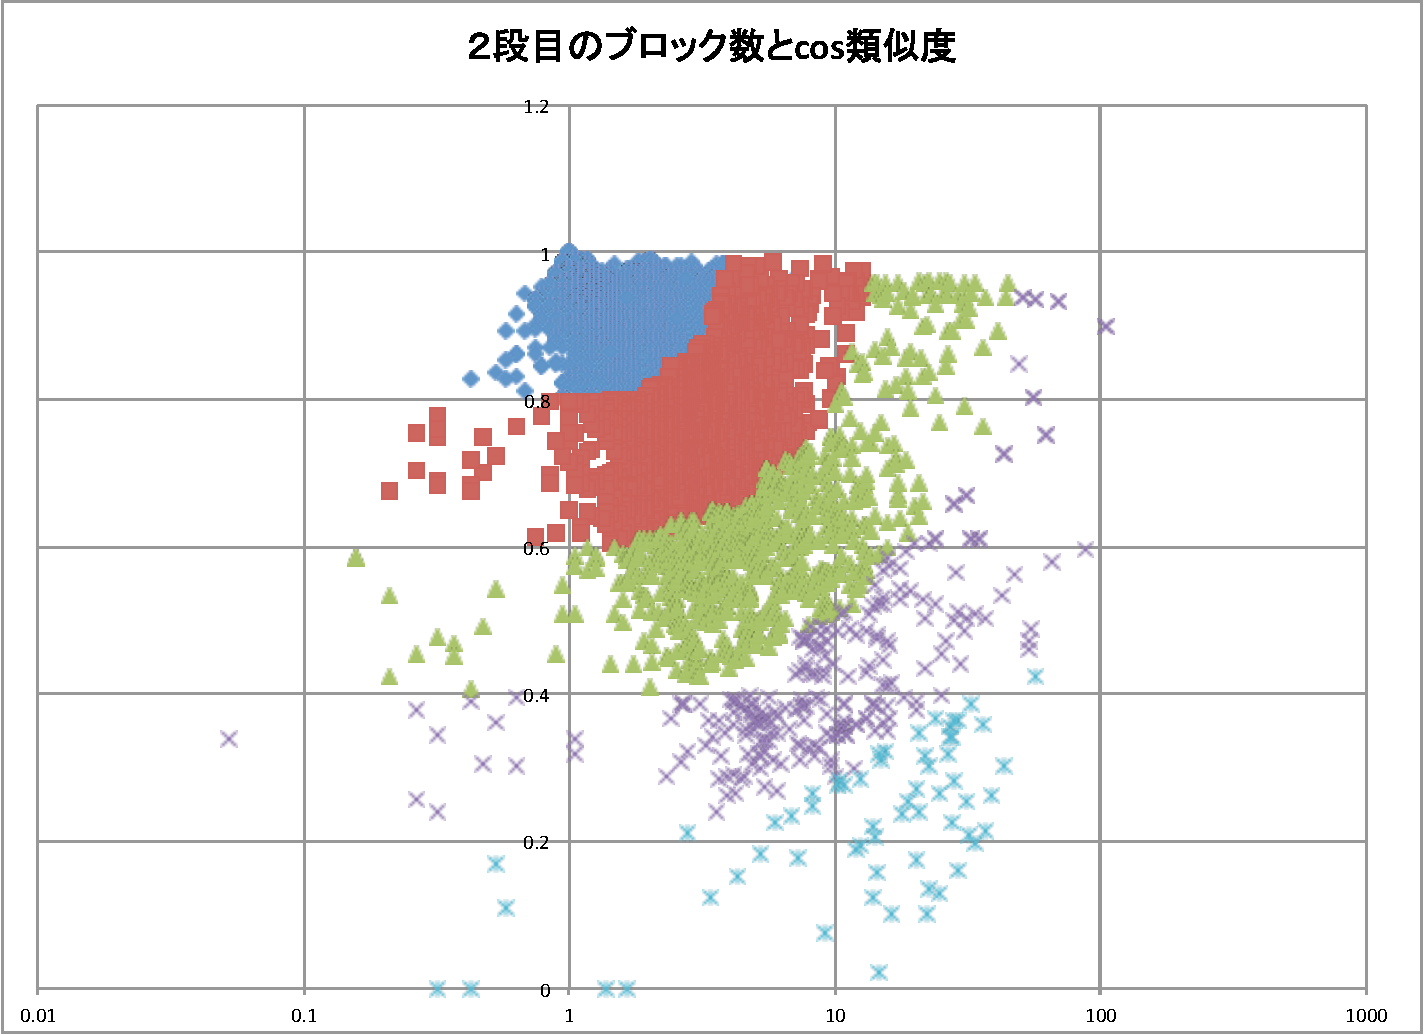
\includegraphics[keepaspectratio, scale = 0.15]{graph_2_block.pdf}
	 \caption{2段目のグラフ}
	 \label{second_block}
	\end{minipage}
 \end{tabular}
  \begin{tabular}{cc}
 	\begin{minipage}[t]{0.45\hsize}
	 \centering
	 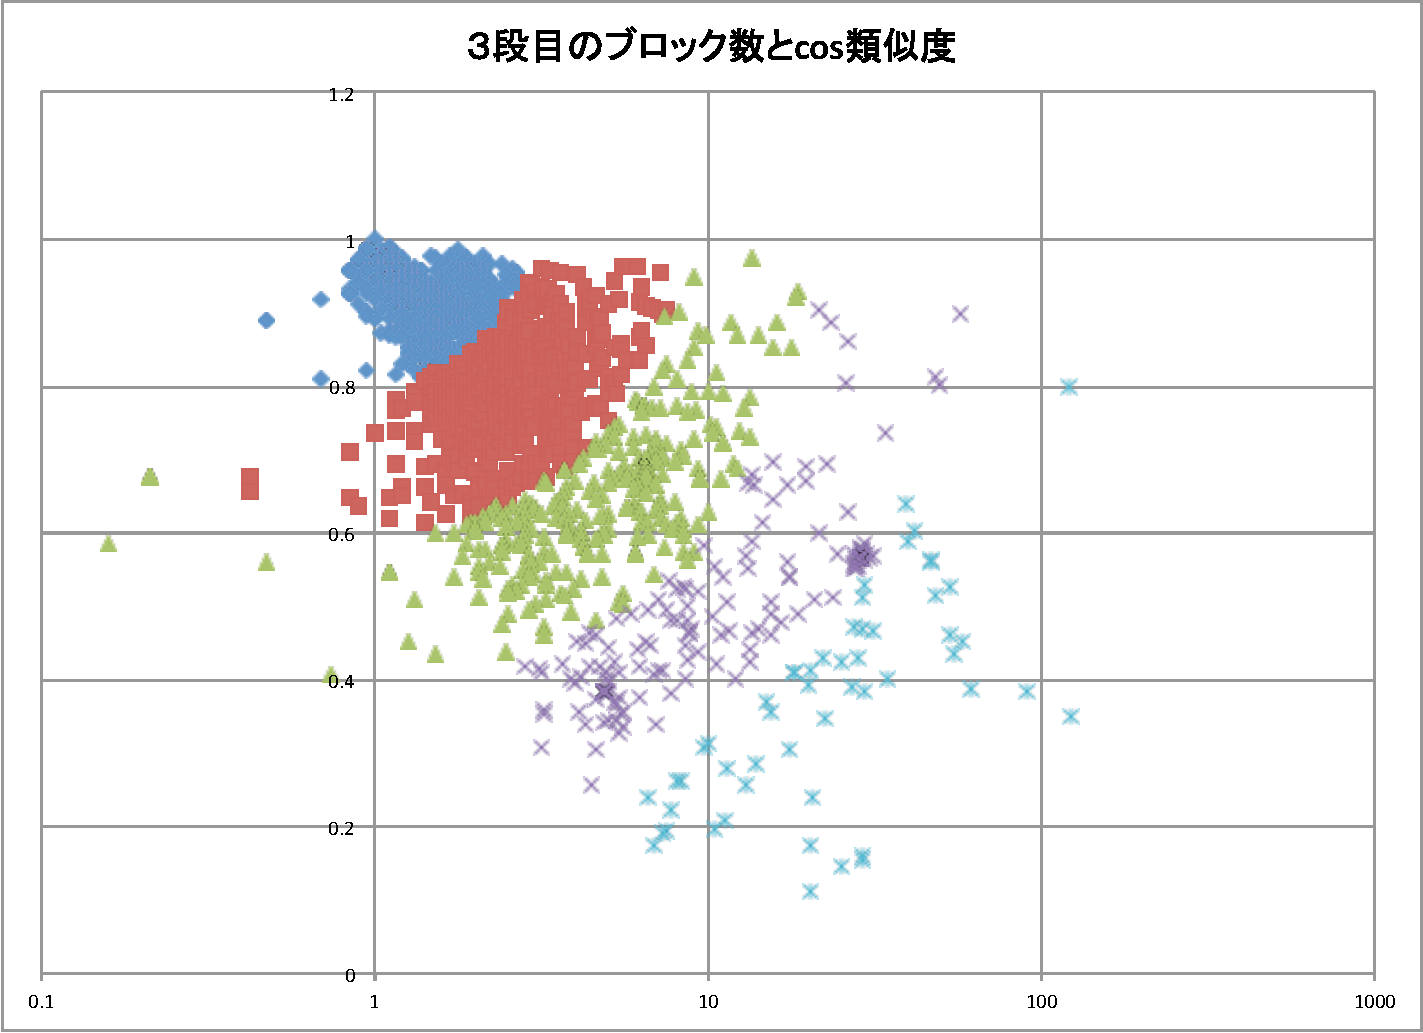
\includegraphics[keepaspectratio, scale = 0.15]{graph_3_block.pdf}
	 \caption{3段目のグラフ}
	 \label{third_block}
	\end{minipage}
        \begin{minipage}[t]{0.45\hsize}
	 \centering
	 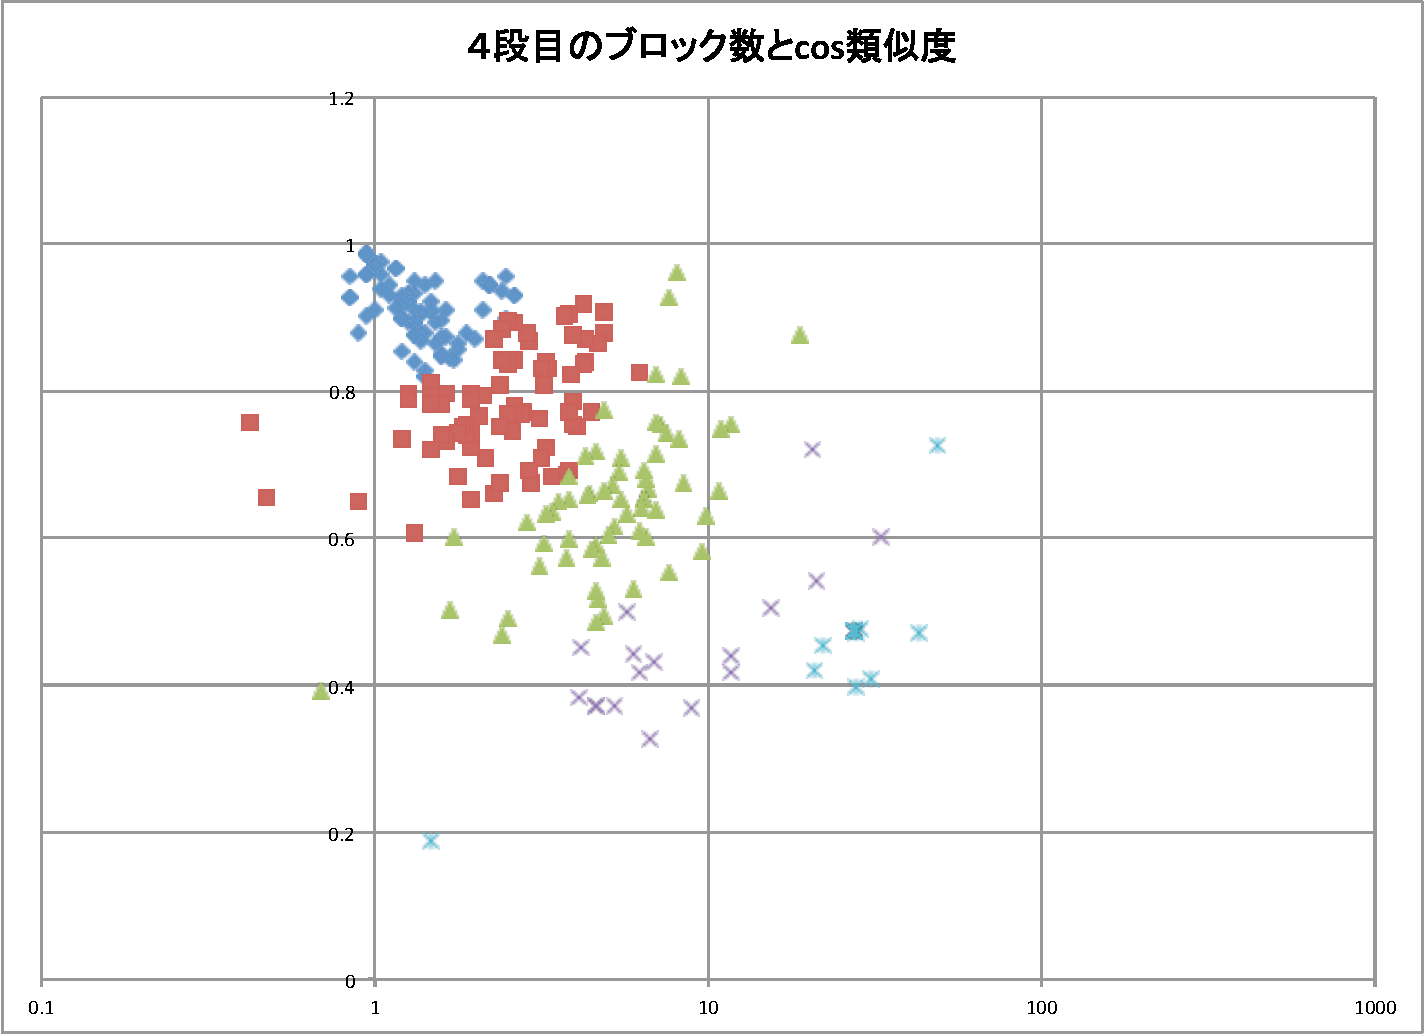
\includegraphics[keepaspectratio, scale = 0.15]{graph_4_block.pdf}
	 \caption{4段目のグラフ}
	 \label{fourth_block}
	\end{minipage}
 \end{tabular}
 \end{figure}

\subsection{スプライト数とcos類似度の散布図}
\begin{figure}[ht]
 \begin{tabular}{cc}
 	\begin{minipage}[t]{0.45\hsize}
	 \centering
	 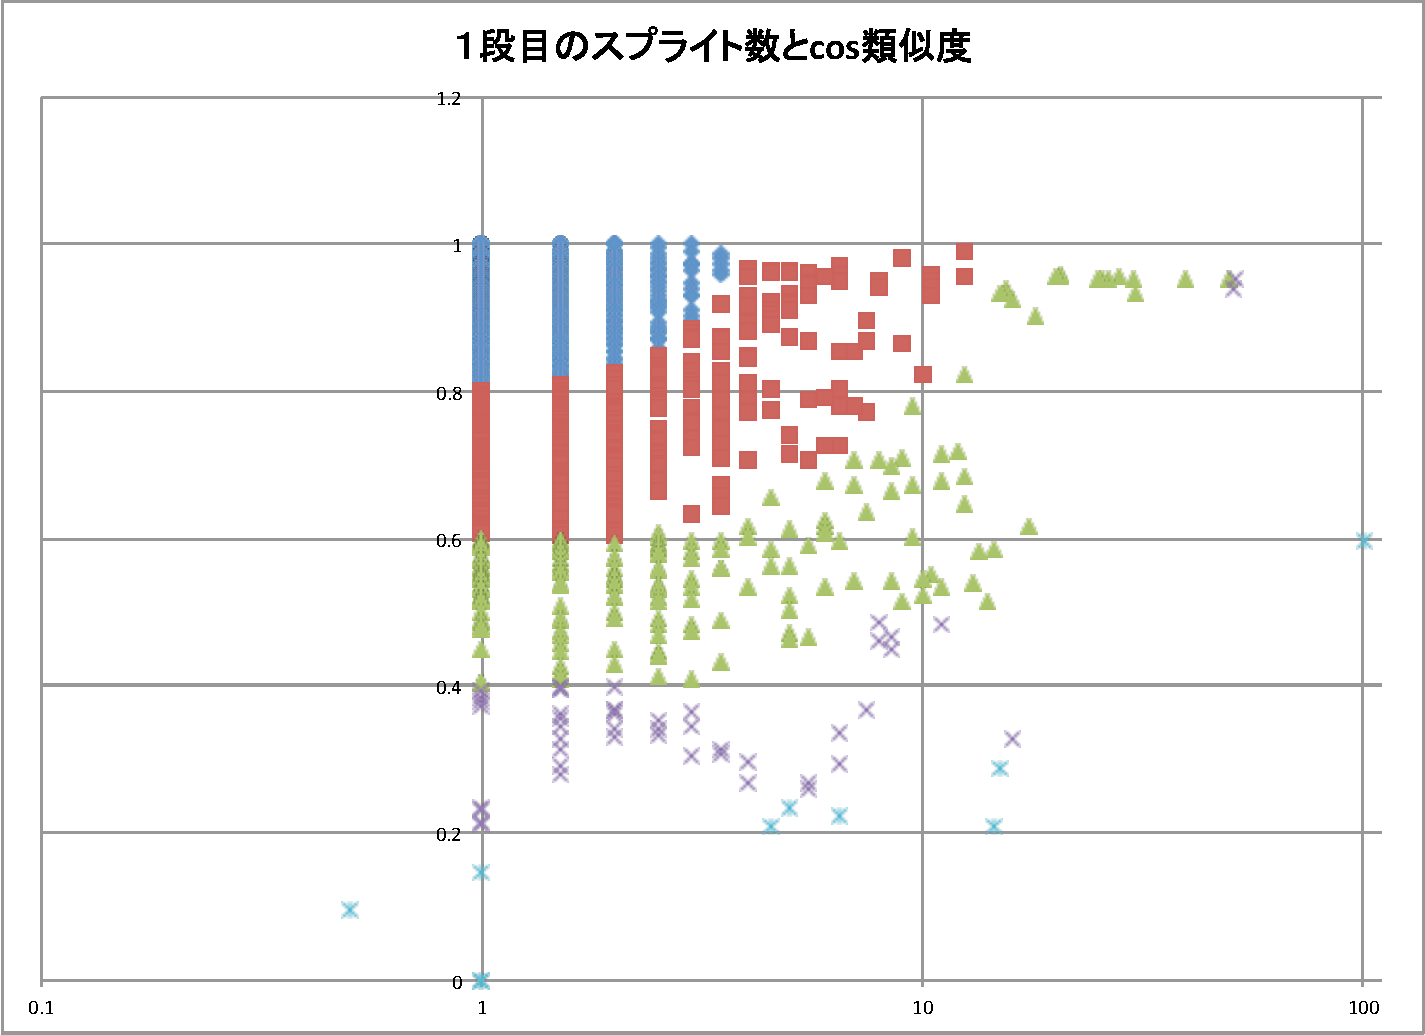
\includegraphics[keepaspectratio, scale = 0.15]{graph_1_splite.pdf}
	 \caption{1段目のグラフ}
	 \label{first_splite}
	\end{minipage}
        \begin{minipage}[t]{0.45\hsize}
	 \centering
	 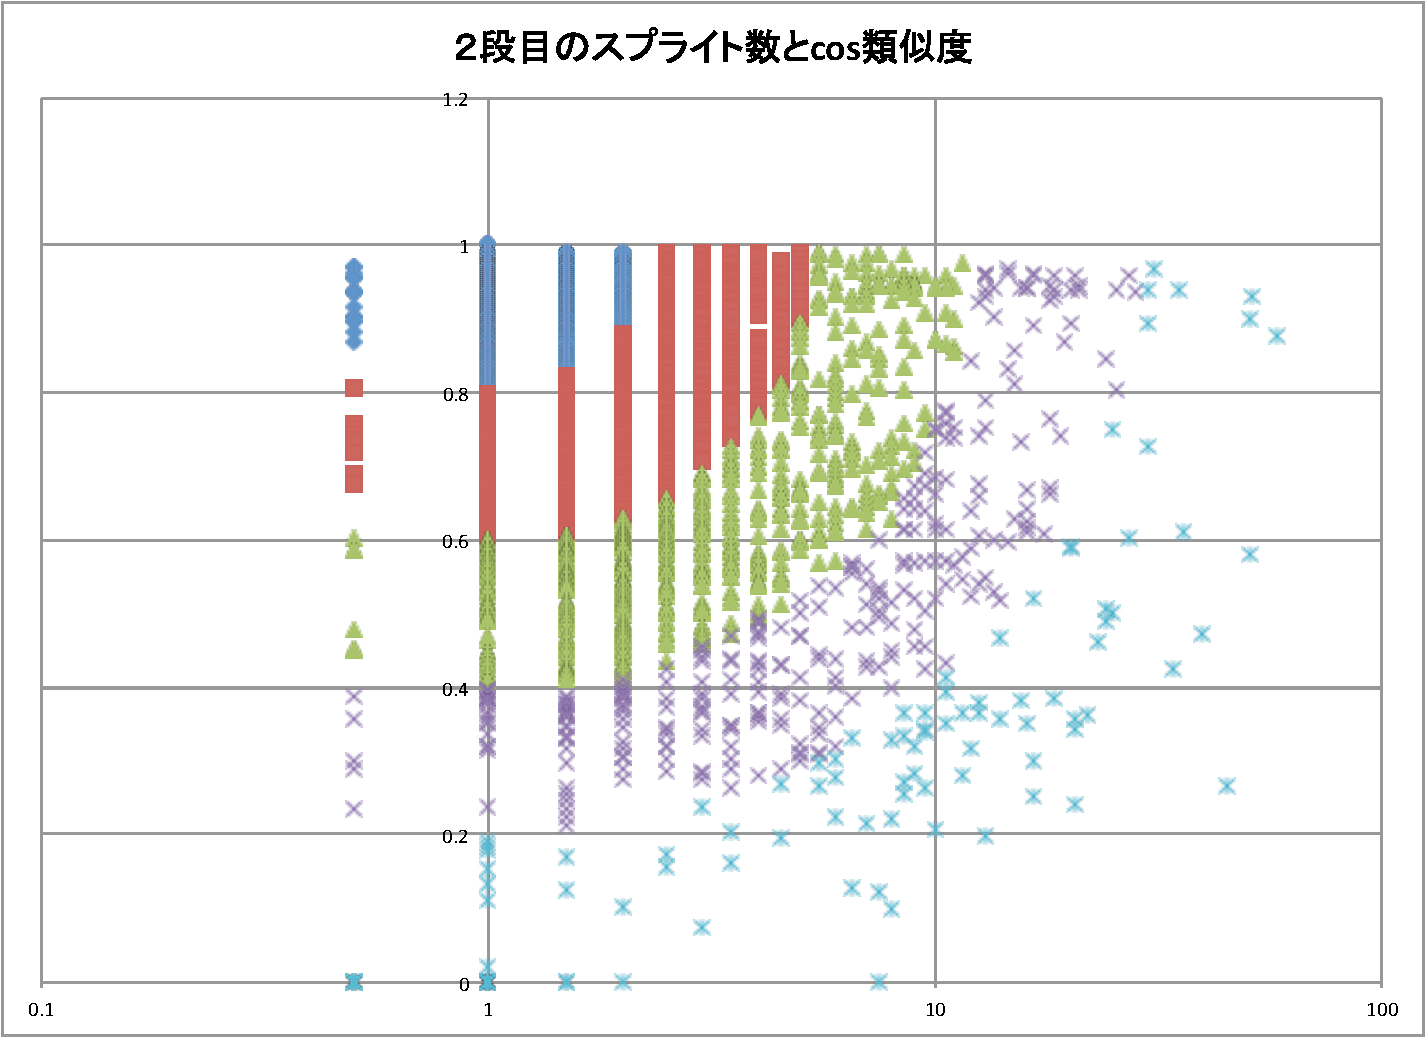
\includegraphics[keepaspectratio, scale = 0.15]{graph_2_splite.pdf}
	 \caption{2段目のグラフ}
	 \label{second_splite}
	\end{minipage}
 \end{tabular}
  \begin{tabular}{cc}
 	\begin{minipage}[t]{0.45\hsize}
	 \centering
	 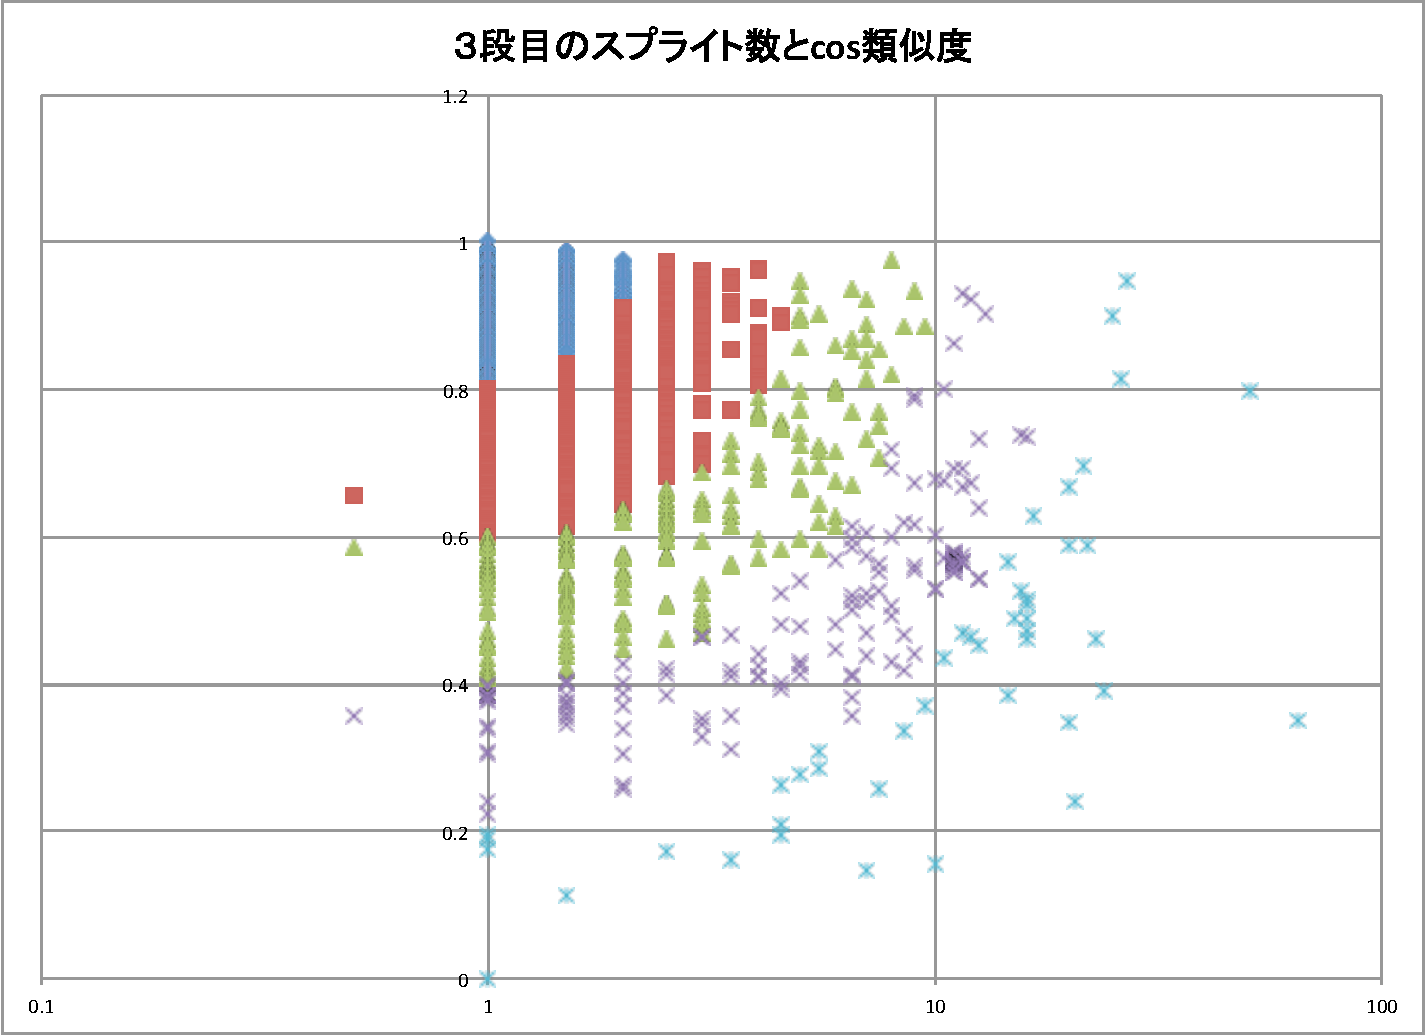
\includegraphics[keepaspectratio, scale = 0.15]{graph_3_splite.pdf}
	 \caption{3段目のグラフ}
	 \label{third_splite}
	\end{minipage}
        \begin{minipage}[t]{0.45\hsize}
	 \centering
	 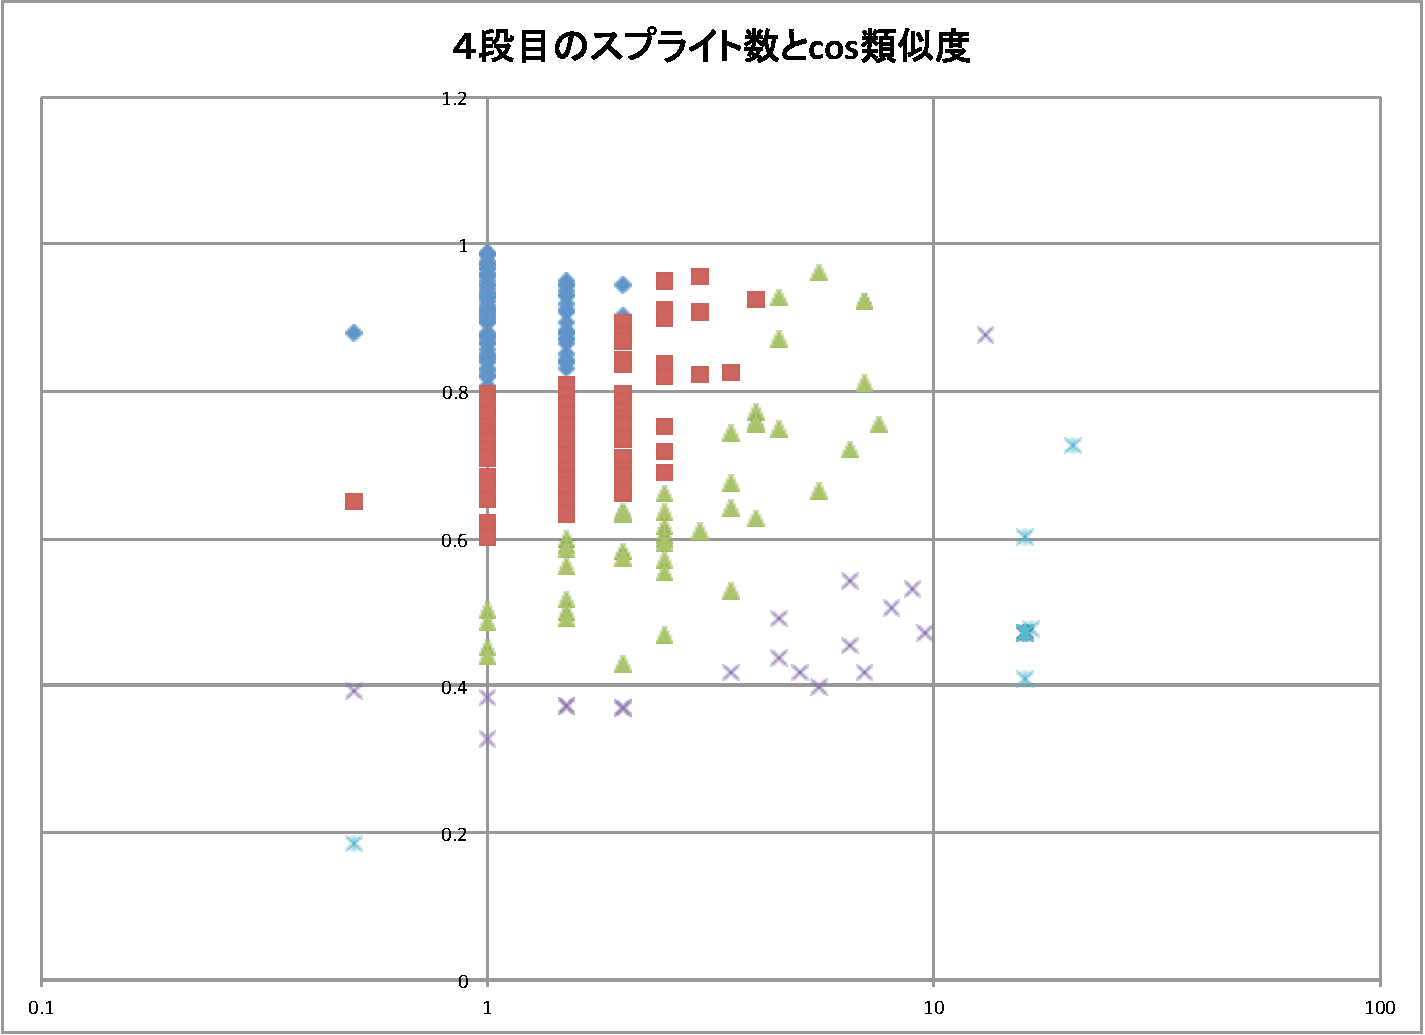
\includegraphics[keepaspectratio, scale = 0.15]{graph_4_splite.pdf}
	 \caption{4段目のグラフ}
	 \label{fourth_splite}
	\end{minipage}
 \end{tabular}
 \end{figure}

\newpage
 \subsection{ブロック数とcos類似度のカラーマップ}
\begin{figure}[ht]
 \begin{tabular}{cc}
 	\begin{minipage}[t]{0.45\hsize}
	 \centering
	 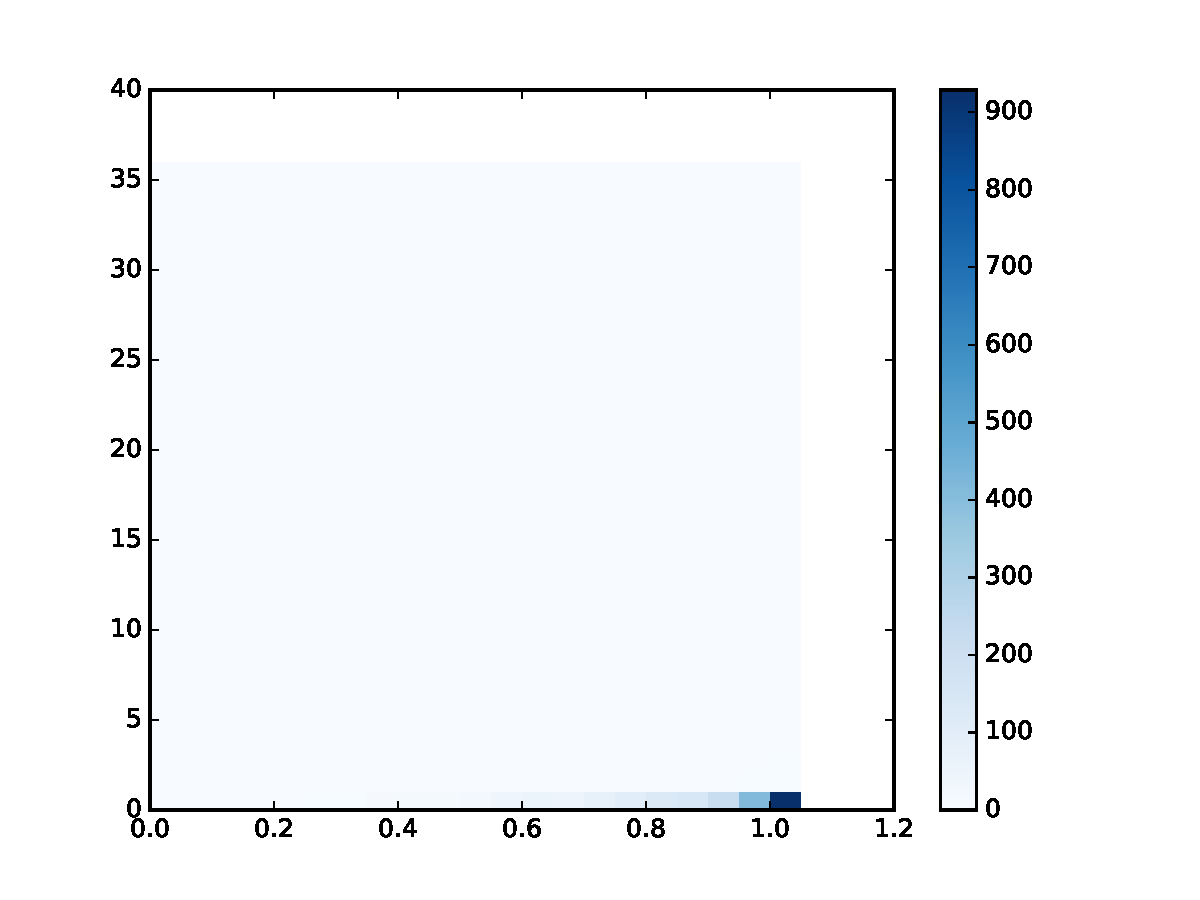
\includegraphics[keepaspectratio, scale = 0.2]{colormap_block_1.pdf}
	 \caption{1段目のグラフ}
	 \label{first_splite}
	\end{minipage}
        \begin{minipage}[t]{0.45\hsize}
	 \centering
	 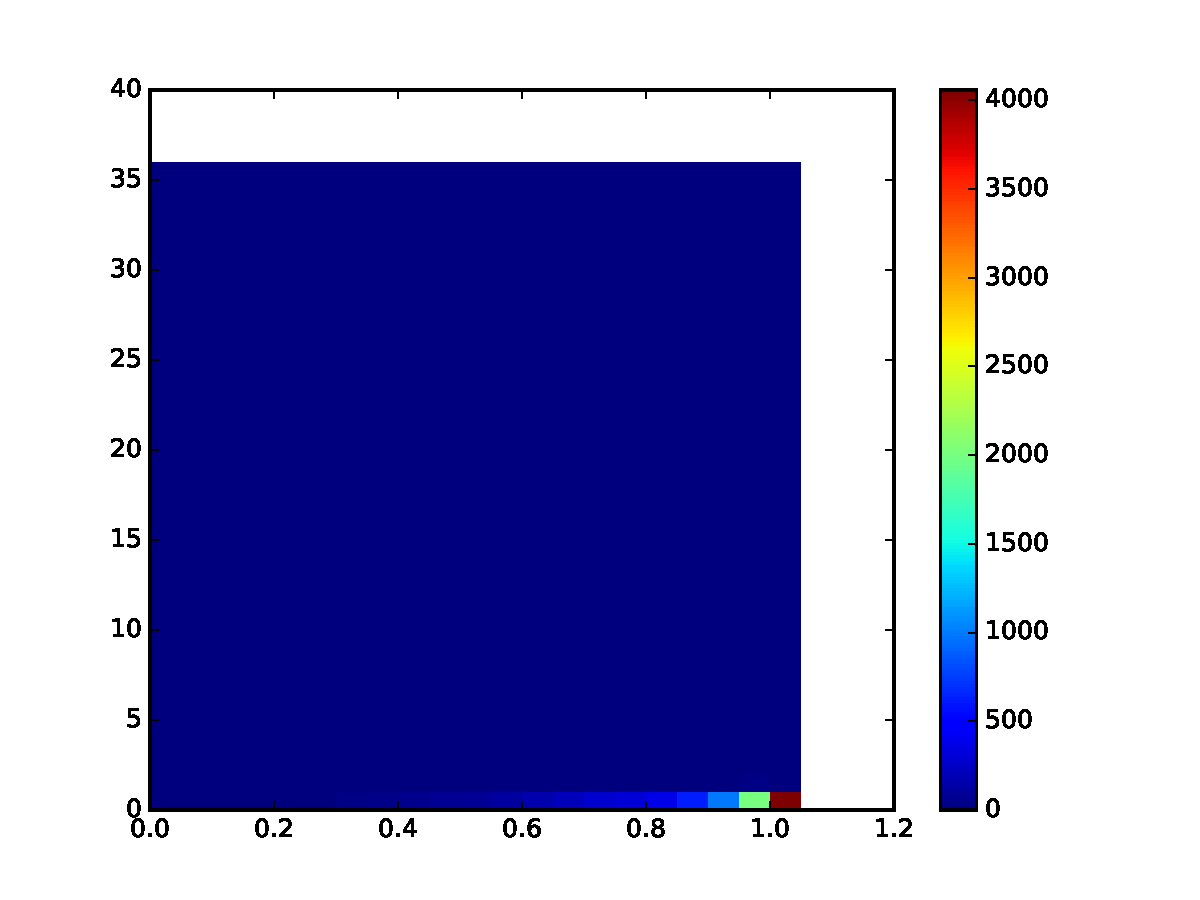
\includegraphics[keepaspectratio, scale = 0.2]{colormap_block_2.pdf}
	 \caption{2段目のグラフ}
	 \label{second_splite}
	\end{minipage}
 \end{tabular}
  \begin{tabular}{cc}
 	\begin{minipage}[t]{0.45\hsize}
	 \centering
	 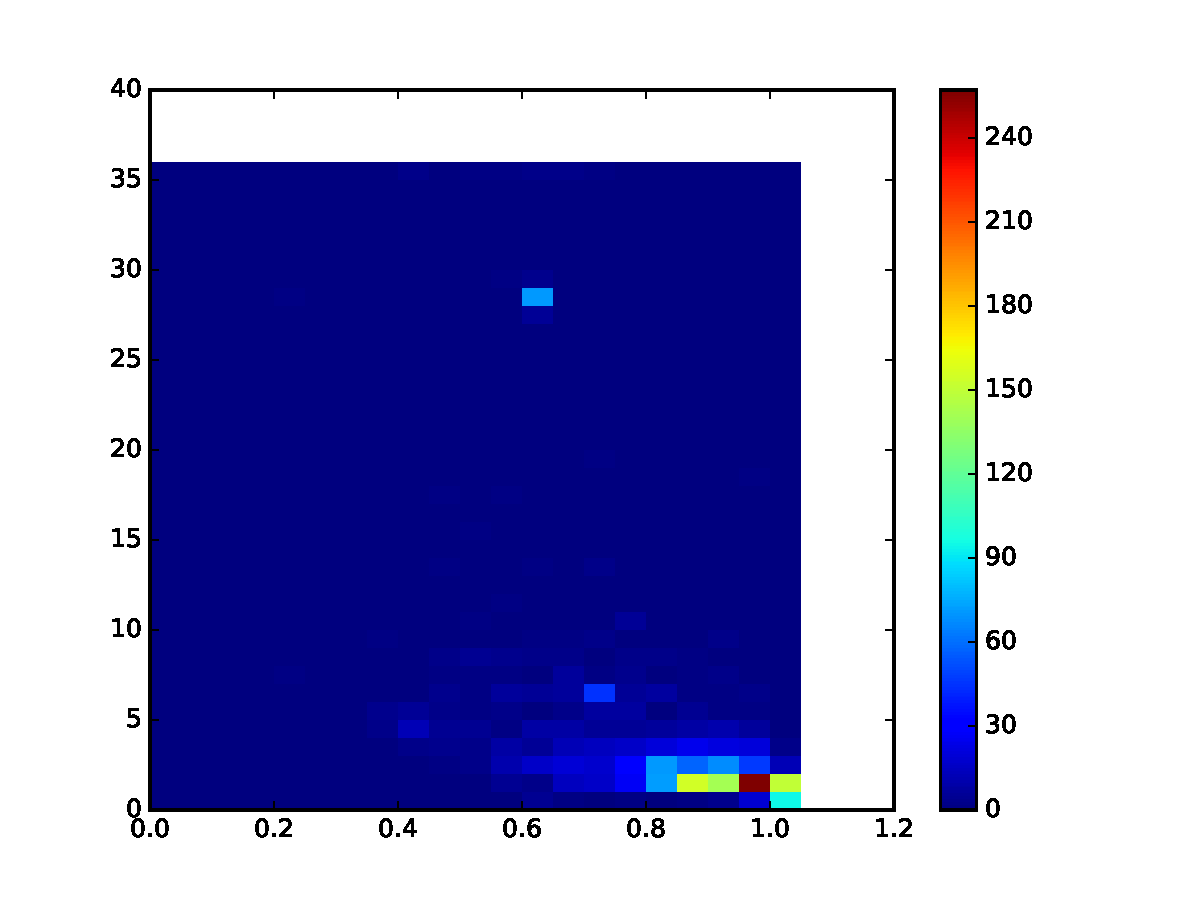
\includegraphics[keepaspectratio, scale = 0.2]{colormap_block_3.pdf}
	 \caption{3段目のグラフ}
	 \label{third_splite}
	\end{minipage}
        \begin{minipage}[t]{0.45\hsize}
	 \centering
	 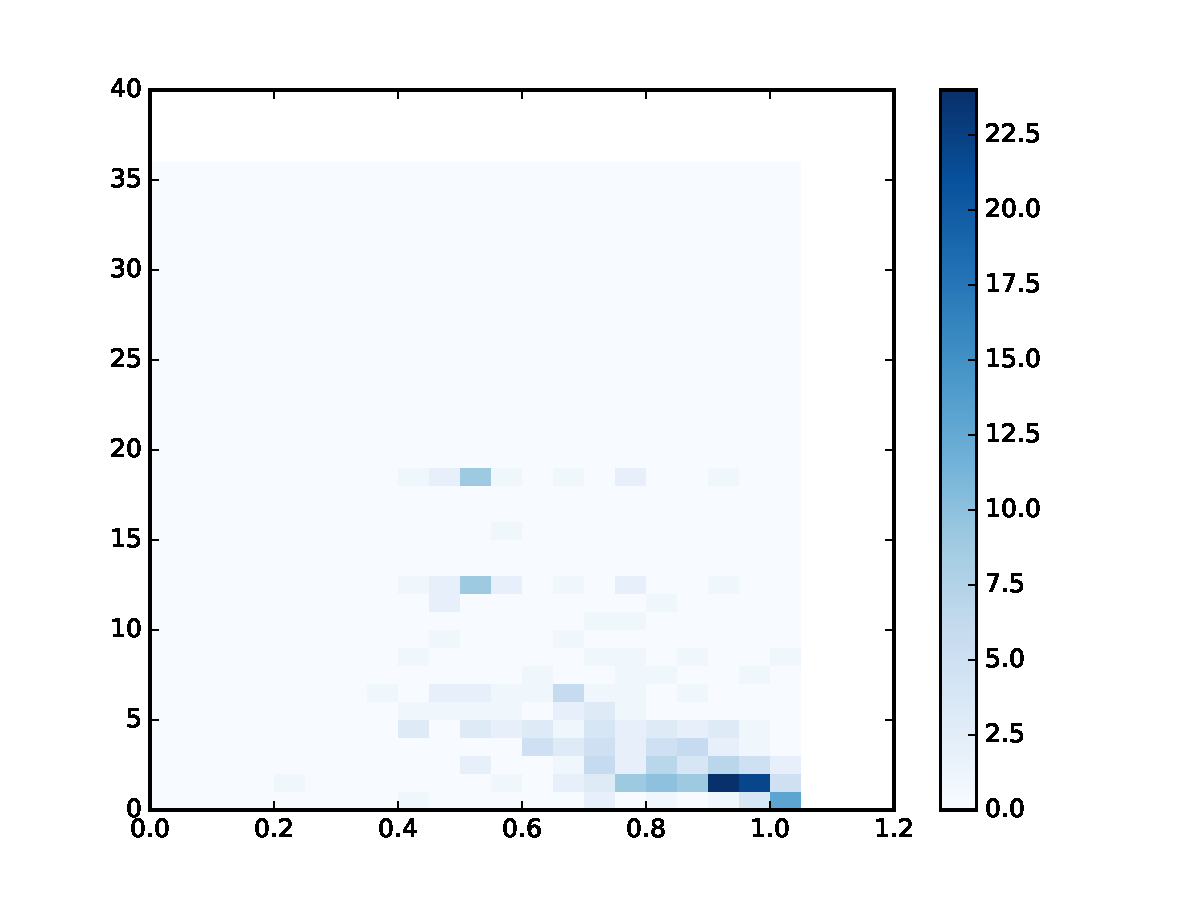
\includegraphics[keepaspectratio, scale = 0.2]{colormap_block_4.pdf}
	 \caption{4段目のグラフ}
	 \label{fourth_splite}
	\end{minipage}
 \end{tabular}
 \end{figure}
 
\subsection{スプライト数とcos類似度のカラーマップ}

\begin{figure}[h]
 \begin{tabular}{cc}
 	\begin{minipage}[t]{0.45\hsize}
	 \centering
	 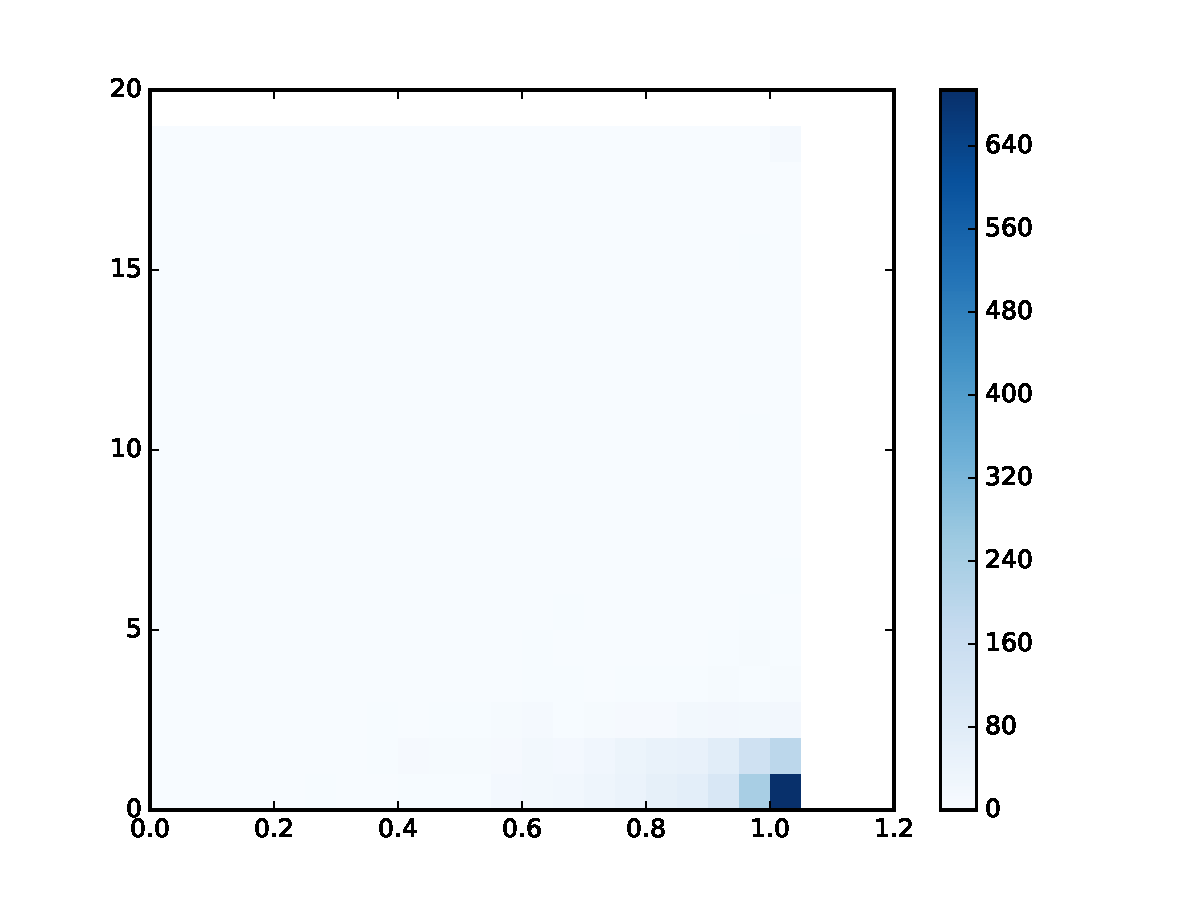
\includegraphics[keepaspectratio, scale = 0.2]{colormap_splite_1.pdf}
	 \caption{1段目のグラフ}
	 \label{first_splite}
	\end{minipage}
        \begin{minipage}[t]{0.45\hsize}
	 \centering
	 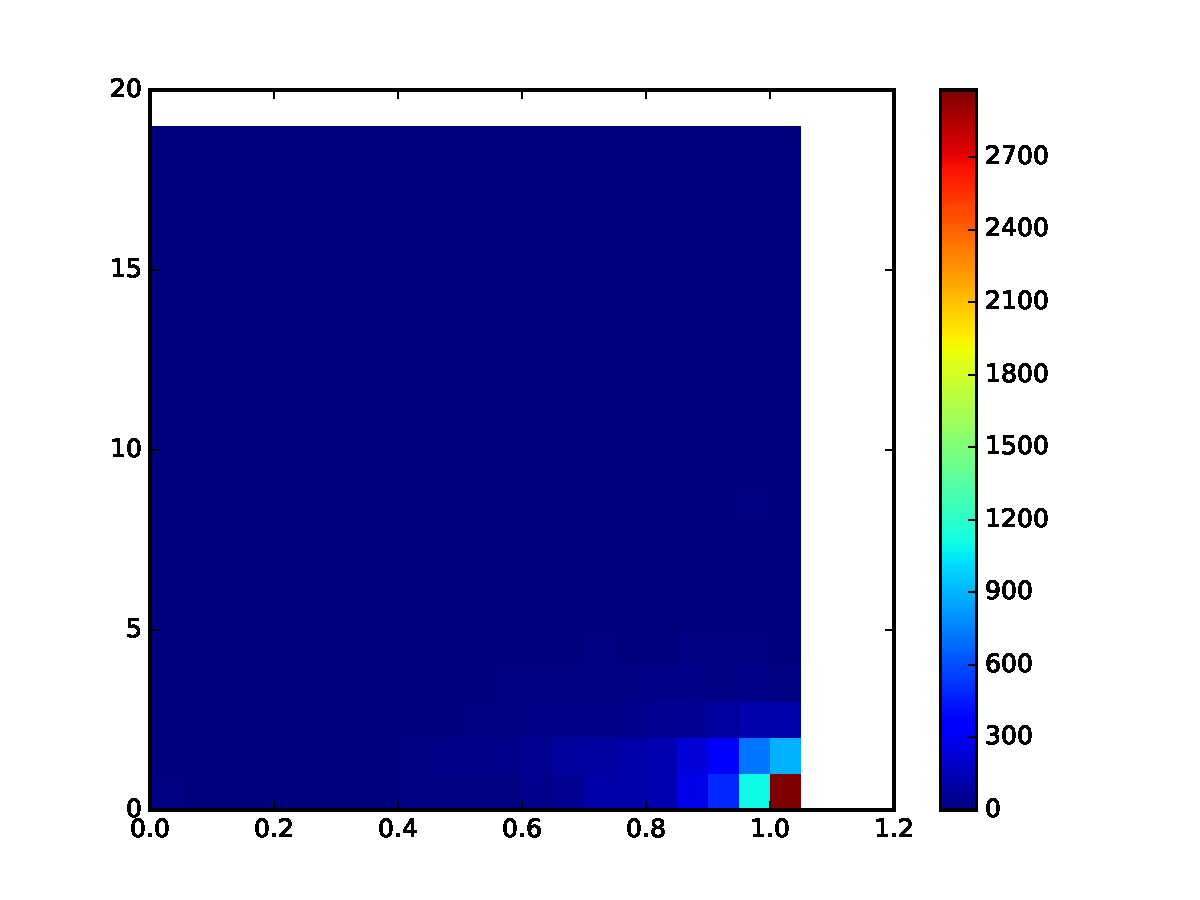
\includegraphics[keepaspectratio, scale = 0.2]{colormap_splite_2.pdf}
	 \caption{2段目のグラフ}
	 \label{second_splite}
	\end{minipage}
 \end{tabular}
  \begin{tabular}{cc}
 	\begin{minipage}[t]{0.45\hsize}
	 \centering
	 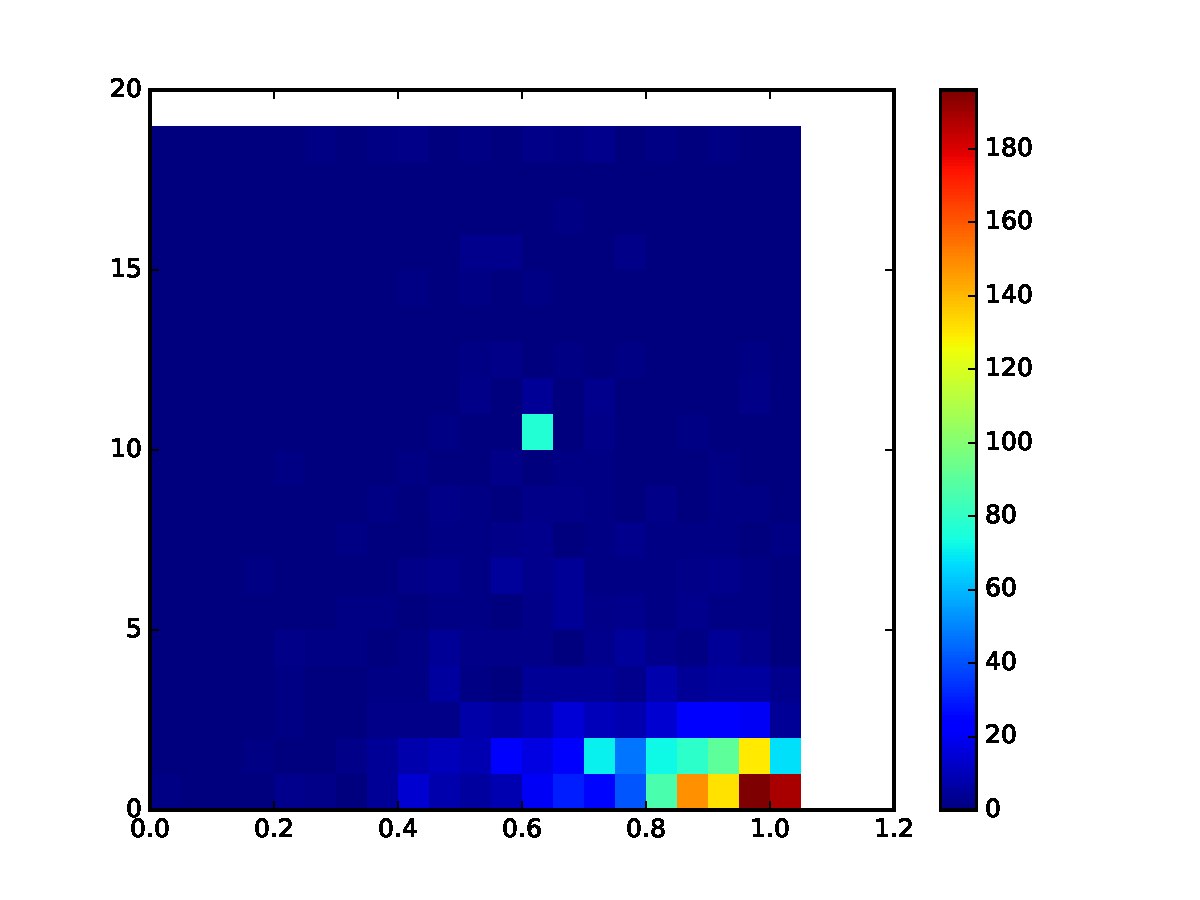
\includegraphics[keepaspectratio, scale = 0.2]{colormap_splite_3.pdf}
	 \caption{3段目のグラフ}
	 \label{third_splite}
	\end{minipage}
        \begin{minipage}[t]{0.45\hsize}
	 \centering
	 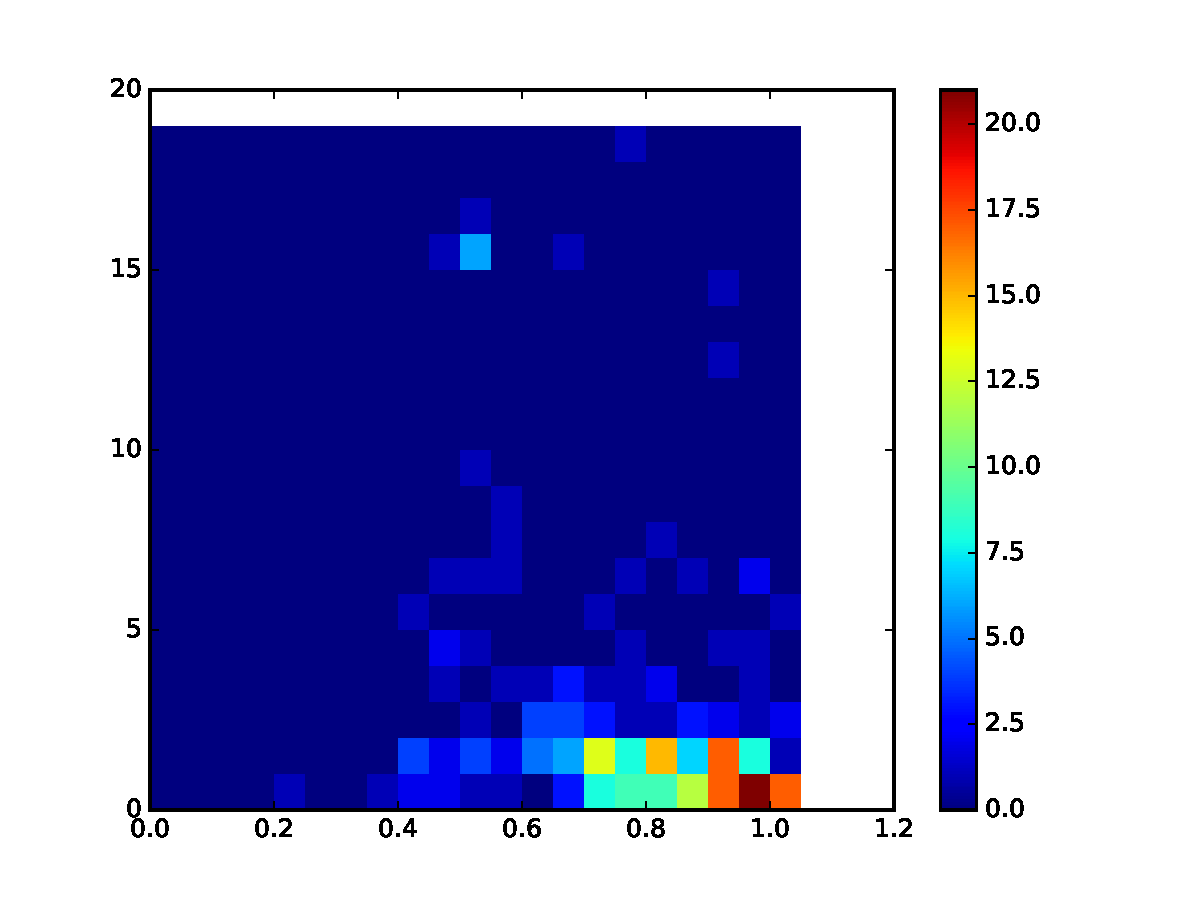
\includegraphics[keepaspectratio, scale = 0.2]{colormap_splite_4.pdf}
	 \caption{4段目のグラフ}
	 \label{fourth_splite}
	\end{minipage}
 \end{tabular}
 \end{figure}

\newpage
\section{評価}


%
%
\end{document}
